\section{Experiments}
We evaluate the VR bound methods on Bayesian neural networks and variational auto-encoders. All the experiments used the ADAM optimizer \cite{kingma:adam}, and the detailed experimental set-up (batch size, learning rate, etc.) can be found in the appendix. The implementation of all the experiments in Python is released at \url{https://github.com/YingzhenLi/VRbound}.

\subsection{Bayesian neural network}

\begin{figure}[t]
 \centering
 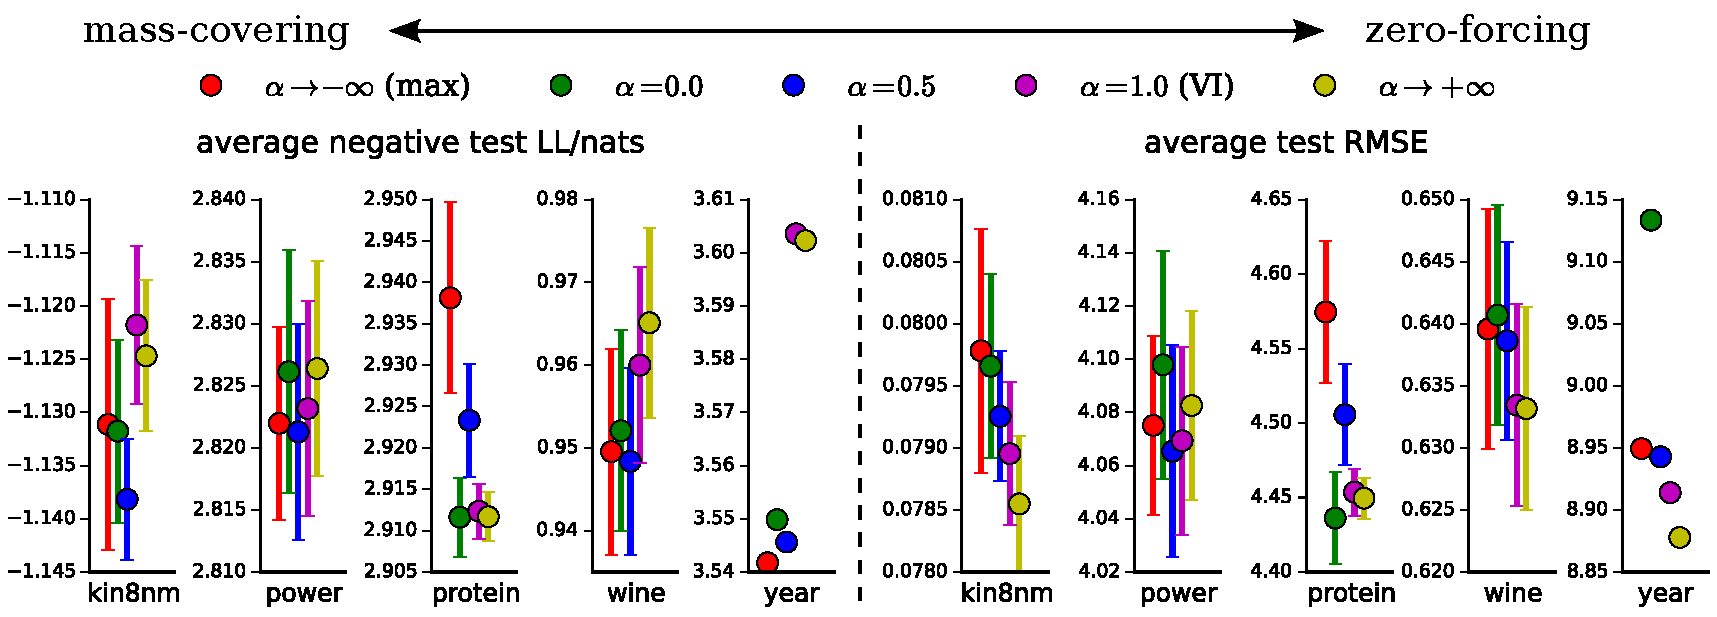
\includegraphics[width=1.0\linewidth]{figs/results_selected_bnn.pdf} 
 \vspace{-0.15in}
 \caption{Test LL and RMSE results for Bayesian neural network regression. The lower the better.}
 \label{fig:bnn_results}
\end{figure}

The first experiment considers Bayesian neural network regression. The datasets are collected from the UCI dataset repository.\footnote{\url{http://archive.ics.uci.edu/ml/datasets.html}} The model is a single-layer neural network with 50 hidden units (ReLUs) for all datasets except Protein and Year (100 units). We use a Gaussian prior $\bm{\theta} \sim \mathcal{N}(\bm{\theta}; \bm{0}, \bm{I})$ for the network weights and Gaussian approximation to the true posterior $q(\bm{\theta}) = \mathcal{N}(\bm{\theta}; \bm{\mu}_q, diag(\bm{\sigma}_q))$. We follow the toy example in Section \ref{sec:vr_bound} to consider $\alpha \in \{-\infty, 0.0, 0.5, 1.0, +\infty \}$ in order to examine the effect of mass-covering/zero-forcing behaviour. Stochastic optimisation uses the energy approximation proposed in Section \ref{sec:large_scale_learning}. MC approximation is also deployed to compute the energy function, in which $K=100, 10$ is used for small and large datasets (Protein and Year), respectively.

We summarise the test negative log-likelihood (LL) and RMSE with standard error (across different random splits except for Year) for selected datasets in Figure \ref{fig:bnn_results}, where the full results are provided in the appendix. These results indicate that for posterior approximation problems, the optimal $\alpha$ may vary for different datasets. Also the MC approximation complicates the selection of $\alpha$ (see appendix). Future work should develop algorithms to automatically select the best $\alpha$ values, although a naive approach could use validation sets. We observed two major trends that zero-forcing/mode-seeking methods tend to focus on improving the predictive error, while mass-covering methods returns better calibrated uncertainty estimate and better test log-likelihood. In particular VI returns lower test log-likelihood for most of the datasets. Furthermore, $\alpha = 0.5$ produced overall good results for both test LL and RMSE, possibly because the skew symmetry is centred at $\alpha = 0.5$ and the corresponding divergence is the only symmetric distance measure in the family.

\subsection{Variational auto-encoder}

The second experiments considers variational auto-encoders for unsupervised learning. We mainly compare three approaches: VAE ($\alpha = 1.0$), IWAE ($\alpha = 0$), and VR-max ($\alpha = -\infty$), which are implemented upon the publicly available code.\footnote{\url{https://github.com/yburda/iwae}}
%
Four datasets are considered: Frey Face (with 10-fold cross validation), Caltech 101 Silhouettes, MNIST and OMNIGLOT. The VAE model has $L=1, 2$ stochastic layers with deterministic layers stacked between, and the network architecture is detailed in the appendix. 
%
We reproduce the IWAE experiments to obtain a fair comparison, since the results in the original publication \cite{burda:iwae} mismatches those evaluated on the publicly available code. 

\begin{figure}[t]
\begin{minipage}{0.6\linewidth}

%\begin{table}[t]
\centering
%\caption
\captionof{table}{ Average Test log-likelihood. Results for VAE on MNIST and OMNIGLOT are collected from \cite{burda:iwae}.}
\label{tab:vae_ll}
\begin{tabular}{lccccc}
\toprule
\bf{Dataset}&$L$&$K$&\bf{ VAE }&\bf{ IWAE }&\bf{ VR-max }\\
\hline
Frey Face&1&5&1322.96&\bf{1380.30}&1377.40\\
($\pm$ std. err.)& & &$\pm$10.03&\bf{$\pm$4.60}&$\pm$4.59 \\
\hline
Caltech 101& 1& 5&-119.69&\bf{-117.89}&-118.01\\
Silhouettes&  &50&-119.61&-117.21&\bf{-117.10}\\
\hline
MNIST& 1&5 &-86.47&\bf{-85.41}&-85.42\\
     &  &50&-86.35&\bf{-84.80}&-84.81\\
     & 2&5 &-85.01&\bf{-83.92}&-84.04\\
     &  &50&-84.78&\bf{-83.05}&-83.44\\
\hline
OMNIGLOT & 1&5 &-107.62&\bf{-106.30}&-106.33\\
		 & 1&50&-107.80&\bf{-104.68}&-105.05\\
		 & 2&5 &-106.31&\bf{-104.64}&-104.71\\
		 & 2&50&-106.30&\bf{-103.25}&-103.72\\
\bottomrule
\end{tabular}
%\end{table}

\end{minipage}
\hfill
\begin{minipage}{0.35\linewidth}
\centering
 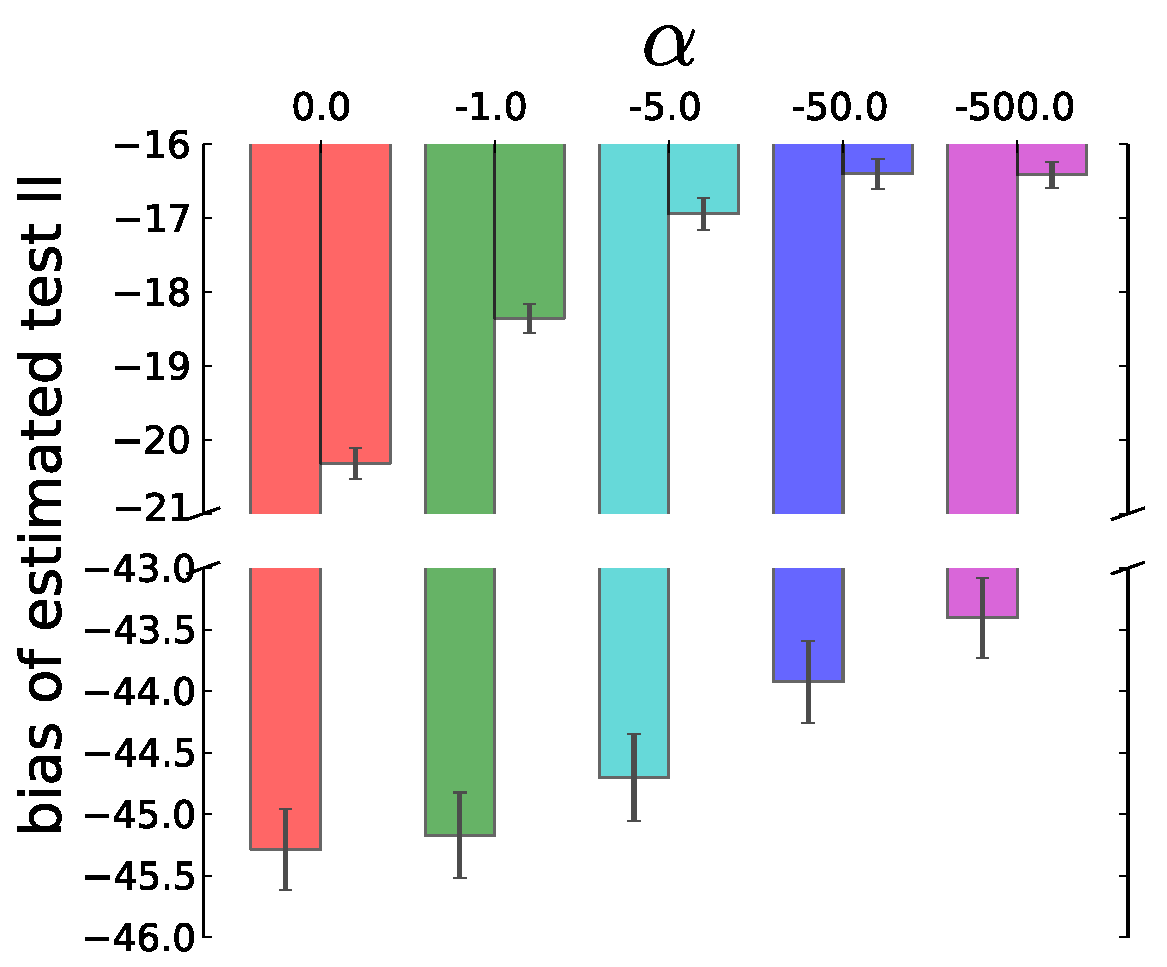
\includegraphics[width=1.00\linewidth]{figs/bias_estimate.pdf} 
 \vspace{-0.1in}
 \captionof{figure}{Bias of sampling approximation to. Results for $K=5, 50$ samples are shown on the left and right, respectively.}
 \label{fig:vae_bias}
\end{minipage}
\vspace{-0.1in}
\end{figure}
\begin{figure*}[!ht]
 \vspace{-0.1in}
 \centering
 \subfigure[Log of ratio $R = w_{max} / (1 - w_{max})$]{
 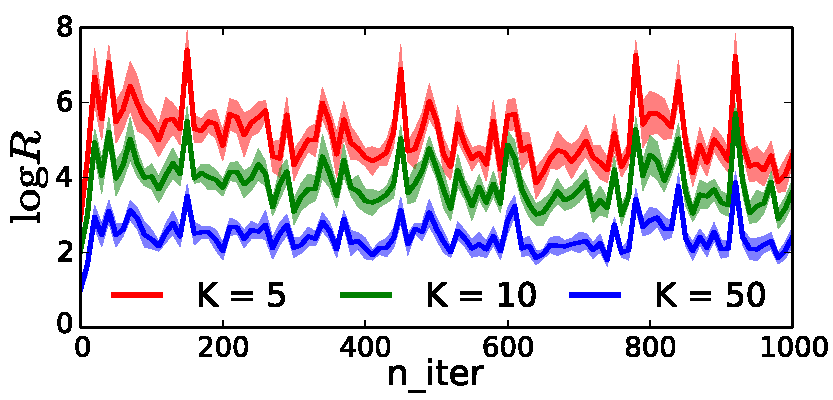
\includegraphics[width=0.37\linewidth]{figs/weight_ratio.pdf}
 \label{fig:weight_ratio}}
 \hspace{0.4in}
 \subfigure[Weights of samples.]{
 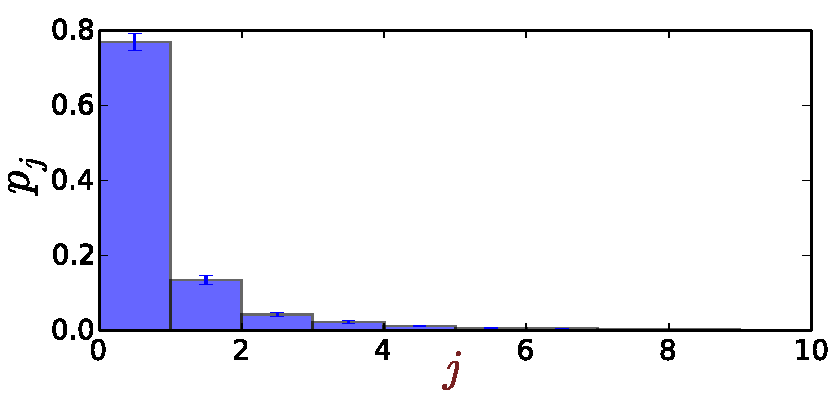
\includegraphics[width=0.37\linewidth]{figs/weight_distribution.pdf}
 \label{fig:weight_distribution}}
\vspace{-0.1in}
 \caption{Importance weights during training, see main text for details. Best viewed in colour.}
 \vspace{-0.1in}
\end{figure*}

We report test log-likelihood results in Table \ref{tab:vae_ll} by computing $\log p(\bm{x}) \approx \hat{\mathcal{L}}_{0, 5000}(q; \bm{x})$ following \cite{burda:iwae}. We also present some samples from the trained models in the appendix. 
%
Overall VR-max is almost indistinguishable from IWAE. Other positive alpha settings (e.g.~$\alpha = 0.5$) return worse results, e.g. $1374.64\pm5.62$ for Frey Face and $-85.50$ for MNIST with $\alpha = 0.5$, $L=1$ and $K=5$. These worse results for $\alpha > 0$ indicate the preference of getting tighter approximations to the likelihood function for MLE problems. Small negative $\alpha$ values (e.g.~$\alpha = -1.0, -2.0$) returns better results on different splits of the Frey Face data, and overall the best $\alpha$ value is dataset-specific. 

VR-max's success might be explained by the tightness of the bound. To evaluate this, we compute the VR bounds on $100$ test datapoints using the 1-layer VAE trained on Frey Face, with $K=\{5, 50\}$ and $\alpha \in \{0, -1, -5, -50, -500 \}$. Figure \ref{fig:vae_bias} presents the estimated gap $\hat{\mathcal{L}}_{\alpha, K} - \hat{\mathcal{L}}_{0, 5000}$. The results indicates that $\hat{\mathcal{L}}_{\alpha, K}$ provides a lower-bound, and that gap is narrowed as $\alpha \rightarrow -\infty$. Also increasing $K$ provides improvements. The standard error of estimation is almost constant for different $\alpha$ (with $K$ fixed), and is negligible when compared to the MC approximation bias.

%
Another explanation for VR-max's success is that, the sample with the largest normalised importance weight $w_{max}$ dominates the contributions of all the gradients.
This is confirmed by tracking $R = \frac{w_{max}}{1 - w_{max}}$ during training on Frey Face (Figure \ref{fig:weight_ratio}). Also Figure \ref{fig:weight_distribution} shows the $10$ largest importance weights from $K=50$ samples in descending order, which exhibit an exponential decay behaviour, with the largest weight occupying more than $75\%$ of the probability mass. Hence VR-max provides a fast approximation to IWAE when tested on CPUs or multiple GPUs with high communication costs. Indeed our numpy implementation of VR-max achieves up to 3 times speed-up compared to IWAE (9.7s vs.~29.0s per epoch, tested on Frey Face data with $K = 50$ and batch size $M = 100$, CPU info: Intel Core i7-4930K CPU @ 3.40GHz). However this speed advantage is less significant when the gradients can be computed very efficiently on a single GPU.